%%%%%%%%%%%%%%%%%%%%%%%%%%%%%%%%%%%%%%%%%%%%%%%%%%%%%%%%%%%%%%%%%%%%%%%%%%%%%%%%%
%
%  Diplomarbeit Vorname Name Datum         
%  "Titel"
%  Lehrstuhl fuer Mustererkennung, FAU Erlangen-Nuernberg
%
%%%%%%%%%%%%%%%%%%%%%%%%%%%%%%%%%%%%%%%%%%%%%%%%%%%%%%%%%%%%%%%%%%%%%%%%%%%%%%%%%

% ++ LME LateX Dokument 
%    Die Verwendung der option "german" bindet german.sty ein.
%    For english papers, use the "english" option and talk to your advisor.
%\documentclass[german,mt]{lmedoc}
\documentclass[english,mt]{lmedoc}

% ++ Umlaut Unterstuetzung
%    Paket "inputenc" kann verwendet werden, um z.B. Umlaute oder das scharfe S
%    direkt (als Nicht-ASCII-Zeichen) einzubinden. Dabei auf die korrekte
%    Kodiermethode achten (z.B. Linux: latin1)! 
\usepackage[latin1]{inputenc}

% ++ es werden keine underfull hboxes als Fehler ausgegeben,
%    da das ja nur hei�t, dass die Seite noch nicht ganz voll ist
\hbadness=10000

%\includeonly{chapters/mt-lit.tex}

\pagenumbering{roman}
\usepackage{natbib}
%\usepackage[backend=bibtex]{biblatex}

%\bibliographystyle{galpha1a} %german bibliography
\bibliographystyle{alphamod} %english bibliographyá
%\bibliographystyle{abnt-num}

\begin{document}
\clearpage
  \begin{deckblatt}
    \Titel{Automatic Detection of Microorganisms from Microscopy Images of Fluid Samples using Machine Learning Techniques}
    \Name{Marti}
    \Vorname{Silvan}
    \Geburtsort{Glarus}
    \Geburtsdatum{09.12.1993}
    \Betreuer{Frauke Wilm}
    \Start{15.03.2022}
    \Ende{15.08.2022}
  \end{deckblatt}


\cleardoublepage

Ich versichere, dass ich die Arbeit ohne fremde Hilfe und ohne Benutzung
anderer als der angegebenen Quellen angefertigt habe und dass die Arbeit
in gleicher oder "ahnlicher Form noch keiner anderen Pr"ufungsbeh"orde
vorgelegen hat und von dieser als Teil einer Pr"ufungsleistung
angenommen wurde. Alle Ausf"uhrungen, die w"ortlich oder sinngem"a"s
"ubernommen wurden, sind als solche gekennzeichnet.
\\

Die Richtlinien des Lehrstuhls f"ur Studien- und Diplomarbeiten
habe ich gelesen und anerkannt, insbesondere die Regelung des
Nutzungsrechts. \\[15mm]
Erlangen, den \selectlanguage{german} \today \hspace{6.0cm} \\[10mm]

\selectlanguage{english} %remove this line for german style

\cleardoublepage

%! Author = silva
%! Date = 6/12/2022

\begin{center}
    \bfseries
    "Ubersicht
    \normalfont
\end{center}
Verschiedene Arten von Bakterien beginnen, Resistenzen gegen einige Arten von Antibiotika zu zeigen, und Studien haben eine Zunahme von Antibiotikaresistenz-assoziierten Krankheiten im Zusammenhang mit diesen nicht erregerspezifischen Therapien gezeigt.
Diese Entwicklungen beg"unstigen den R"uckgriff auf erregerspezifische Ans"atze, erfordern jedoch einen hohen manuellen Aufwand und sind dadurch arbeits- und zeitintensiv.
In dieser Hinsicht k"onnten Mittel zum Nachweis des Bakterientyps durch Analyse mikroskopischer Bilder von Fl"ussigkeitsproben unter Verwendung moderner Bildverarbeitungs- und maschineller Lernwerkzeuge die unerschwinglichen Kosten manueller Methoden vermeiden.
Daher wollen diese Strategien untersucht werden, um das Problem der automatischen Objekterkennung in mikroskopischen Bildern von Fl"ussigkeitsproben anzugehen.

Translate this page



\vspace{5.0cm}

\begin{center}
    \bfseries
    Abstract
    \normalfont

\end{center}

    Various types of bacteria are starting to show resistance against some types of antibiotics and studies have shown an increase in antibiotic-resistance-associated diseases linked to these non-pathogen-specific therapies.
    These developments encourage reverting to pathogen-specific approaches however It requires a high amount of manual work and is thereby laborious and time-consuming.
    In this regard, means to detect the type of bacteria by analysing microscopic images of fluid samples using modern image processing and machine learning tools could avoid the prohibitive costs of manual methods.
    Therefore, want to investigate these strategies to address the problem of automatic object detection in microscopic images of fluid samples.
\cleardoublepage

\tableofcontents

\cleardoublepage \pagenumbering{arabic}

%! Author = silva
%! Date = 6/6/2022


\chapter{Introduction}\label{ch:intro}



The images were obtained to better understand Parkinson's disease.


\section{Datasets}\label{sec:dataset}

We have two datasets of microscopy images which both consist of several ten thousands.
Once we have "cell_type_1" and "cell_type_2".


\captionsetup{labelformat=empty}
\begin{figure}[ht!]
    \begin{minipage}[t]{\linewidth}
        \centering
        \begin{minipage}[t]{0.49\linewidth}
            
\includegraphics[width=\textwidth, keepaspectratio]{./graphics/dataset_sample_1.png}  %  <<< image name 1
        \end{minipage}
        \begin{minipage}[t]{0.49\linewidth}
            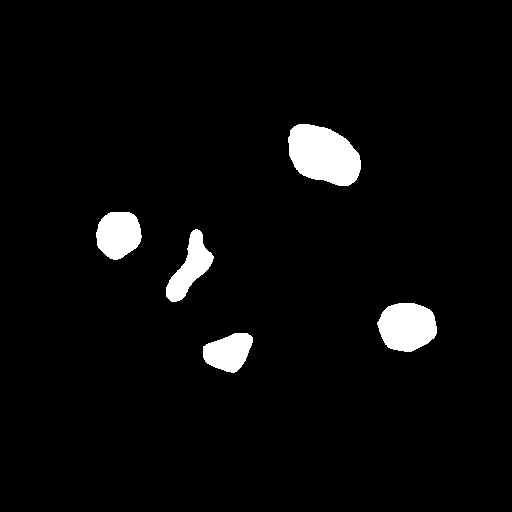
\includegraphics[width=\textwidth, keepaspectratio]{./graphics/dataset_sample_1_label.png}  %  <<< image name 1
        \end{minipage}
    \end{minipage}

    \begin{minipage}[t]{\linewidth}
        \begin{minipage}[t]{0.49\linewidth}
            
\includegraphics[width=\textwidth, keepaspectratio]{./graphics/dataset_sample_2.png}  %  <<< image name 1
        \end{minipage}
        \begin{minipage}[t]{0.49\linewidth}
            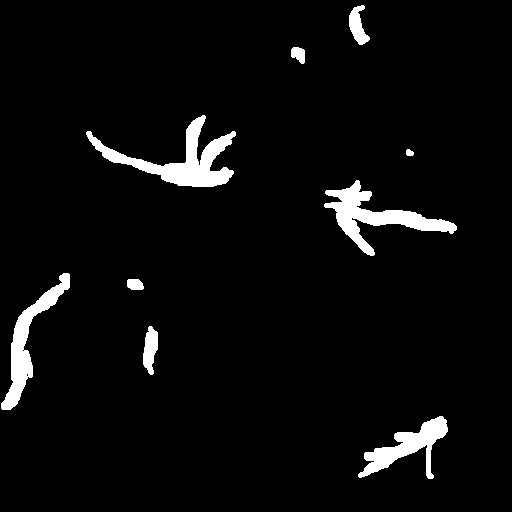
\includegraphics[width=\textwidth, keepaspectratio]{./graphics/dataset_sample_2_label.png}  %  <<< image name 1
        \end{minipage}
    \end{minipage}
    \label{fig:1}
    \caption{Dataset 2: Datasets }
\end{figure}


\section{haha2}

% Einfuehrung (\chapter{Einf"uhrung})
\cleardoublepage
%! Author = silva
%! Date = 6/6/2022


\chapter{Methods}   % (\chapter{})
\cleardoublepage
%! Author = silva
%! Date = 6/6/2022


\chapter{Results}   % (\chapter{})
\cleardoublepage
%! Author = silva
%! Date = 6/6/2022


\chapter{Discussion}   % (\chapter{})
\cleardoublepage
%! Author = silva
%! Date = 6/6/2022

\addcontentsline{toc}{chapter}{Conclusion}
\chapter{Conclusion}

haha \cite{Doerrer87:ELS} hoho \cite[dfdf]{Rodler01:EEF} hihi \cite{Hallinan99:DOM} huhu \cite{Bamford96:AWI}   % (\chapter{})
\cleardoublepage
%! Author = silva
%! Date = 6/6/2022


\chapter{06}   % (\chapter{})
\cleardoublepage
%! Author = silva
%! Date = 6/6/2022


\chapter{07}   % Ausblick (\chapter{Ausblick} TEXT)
\cleardoublepage
%! Author = silva
%! Date = 6/6/2022


\chapter{08}   % Zusammenfassung (\chapter{Zusammenfassung}  TEXT)
\cleardoublepage

\appendix
\cleardoublepage
%! Author = silva
%! Date = 6/6/2022


\chapter{09}   % Glossar (\chapter{Glossar}  TEXT)
\cleardoublepage

%%%%%%%%%%%%%%%%%%%%%%%%%%%%%%%%%%%%%%%%%%%%%%%%%%%%%%%%%%%%%%%%%%%%%%%%%%
% Diese Datei nicht veraendern!
%%%%%%%%%%%%%%%%%%%%%%%%%%%%%%%%%%%%%%%%%%%%%%%%%%%%%%%%%%%%%%%%%%%%%%%%%%
\addcontentsline{toc}{chapter}{\listfigurename}
\listoffigures
 % Bilderverzeichnis
\cleardoublepage
%%%%%%%%%%%%%%%%%%%%%%%%%%%%%%%%%%%%%%%%%%%%%%%%%%%%%%%%%%%%%%%%%%%%%%%%%%
% Diese Datei nicht veraendern!
%%%%%%%%%%%%%%%%%%%%%%%%%%%%%%%%%%%%%%%%%%%%%%%%%%%%%%%%%%%%%%%%%%%%%%%%%%
\addcontentsline{toc}{chapter}{\listtablename}
\listoftables
 % Tabellenverzeichnis
\cleardoublepage
%%%%%%%%%%%%%%%%%%%%%%%%%%%%%%%%%%%%%%%%%%%%%%%%%%%%%%%%%%%%%%%%%%%%%%%%%%
% Diese Datei nicht veraendern!
%%%%%%%%%%%%%%%%%%%%%%%%%%%%%%%%%%%%%%%%%%%%%%%%%%%%%%%%%%%%%%%%%%%%%%%%%%
\addcontentsline{toc}{chapter}{\bibname}
\bibliography{chapters/mt}
 % Literaturverzeichnis
\cleardoublepage

\end{document}
